\documentclass{article}
\usepackage[utf8]{inputenc}
\usepackage[T2A]{fontenc}
\usepackage[utf8]{inputenc}
\usepackage{float}
%\usepackage[russian]{babel}
\usepackage[a4paper, left=10mm, right=10mm, top=20mm, bottom=20mm]{geometry}
\usepackage{natbib}
\usepackage{graphicx}
\usepackage{tabularx}
\usepackage{hyperref}

\title{PSD@CBM firmware description (draft, for internal use)}
\author{Finogeev Dmitry, INR RAS}





\begin{document}

\maketitle

Actual version of the document is avaliable at github:
\newline
\url{https://github.com/dfinogee/PSD-readout-manual/raw/main/PSD_readout_manual.pdf}



\tableofcontents

\newpage

\section{ADC data processing}
PSD\_data\_readout component receive data from all ADCs, process waveform and output data in GBT packets. Schematic of component is presented on fig.~\ref{fig:1}.

\begin{figure}[H]
	\centering 
	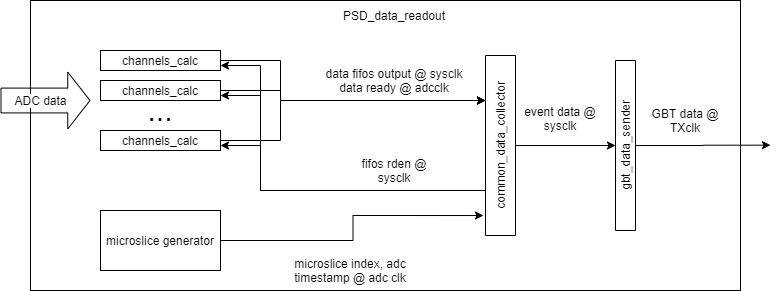
\includegraphics[width=0.8\textwidth]{ADC_readout.png}
	\caption{\label{fig:1} ADC data readout scheme}
\end{figure}




\subsection{Component channels\_calc}
Channel\_calc component scheme is presented on figure~\ref{fig:2}. ADC data inverted for negative signals, zero level and RMS are calculated and avaliable from slow control.


\begin{figure}[H]
	\centering 
	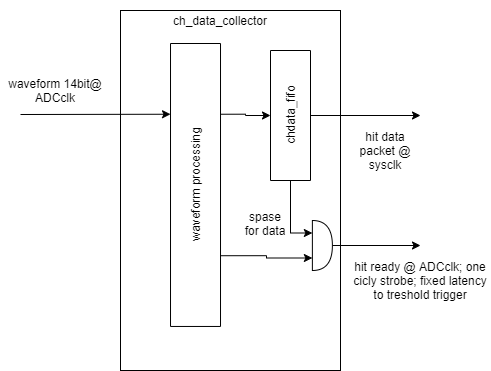
\includegraphics[width=1.0\textwidth]{ADC_event_collection.png}
	\caption{\label{fig:2} Channel data processing scheme}
\end{figure}


Strobe\_generator component forms waveform gate, start and stop signals by threshold crossing taking waveform length and offset parameters. Waveform data that are available from the start (zero level) are latched while strobe. Signal diagram of the component is presented on figure~\ref{fig:3}

\begin{figure}[H]
	\centering 
	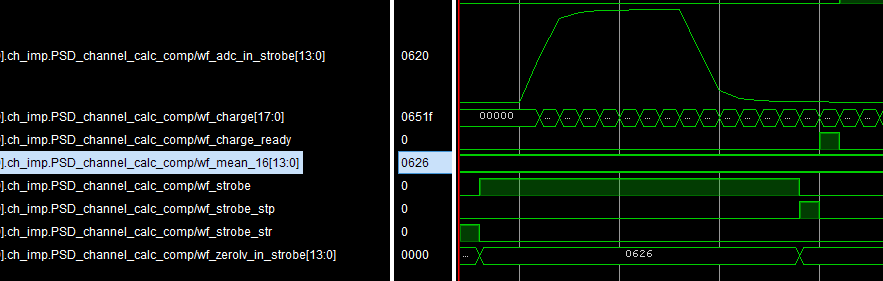
\includegraphics[width=0.8\textwidth]{wf_strobe_diag.png}
	\caption{\label{fig:3} Signal waveform strobe (length 16, offset 3)}
\end{figure}


Ch\_data\_collector store waveform point in raw\_fifo by strobe signal and start waveform data (zero level) by start signal. When charge ready signal raised, charge and start data from header\_fifo stored in data\_fifo as hit packed header. This allow to upgrade charge calculation with fitting procedure and change calculation delay. In next cycle waveform points are read from raw\_fifo and (if sending wf points parameter is set on) stored as hit data in ch\_data\_fifo. After hit packet stored, ready signal raised or dropped signal in case fifo was full and hit packet was dropped. Ready and dropped signals are synchronous to threshold crossing and used for event ADC timestamp.  Signals diagramm of the component is presented on figure~\ref{fig:4}.


\begin{figure}[H]
	\centering 
	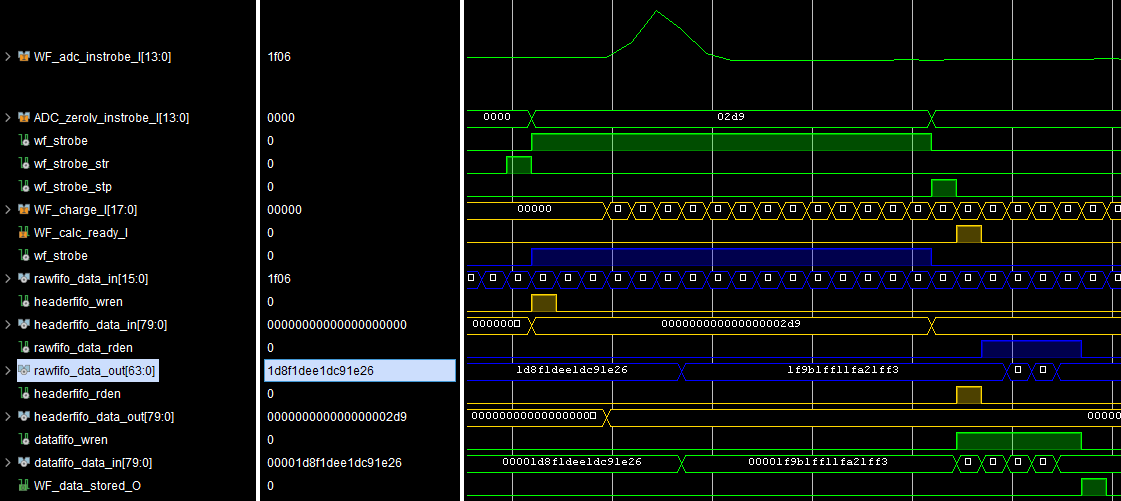
\includegraphics[width=1.0\textwidth]{ADC_ch_data_collector_wave.png}
	\caption{\label{fig:4} Channel data collecting signals}
\end{figure}

Signals could be processed one after another without dead time. If next adc point after waveform gate is higher than threshold, new signal gate is formed. Signal time is next adc cycle after first gate, not is real time of second waveform threshold crossing. Signal diagram for such case is presented on figure~\ref{fig:5}.


\begin{figure}[H]
	\centering 
	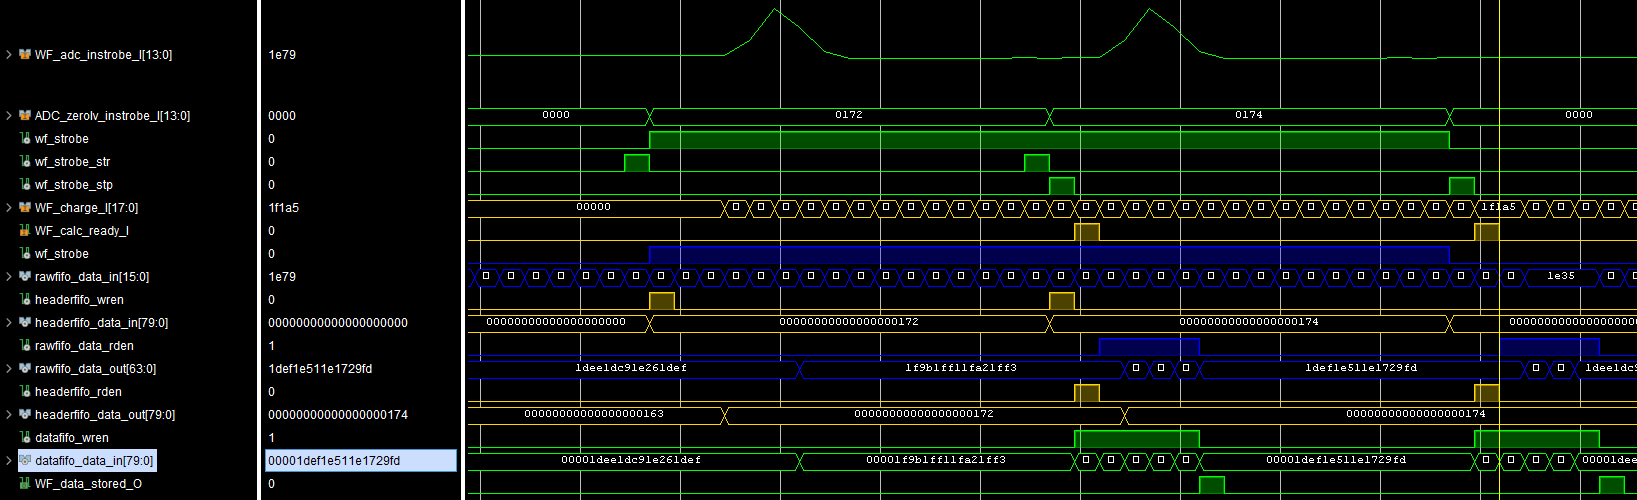
\includegraphics[width=1.0\textwidth]{ADC_ch_data_collector_wave_pileup.png}
	\caption{\label{fig:5} Channel data collecting signals}
\end{figure}

\subsection{Component common\_data\_collector}
Each channel generate single strobe with fixed latency to threshold crossing indicating waveform measurement. 32 bit strobe word is stored to data\_wf\_calc\_fifo with mc index and ADC timestamp. FSM read stored strobes and collect data from fired channels storing outputs to common\_data\_fifo, each event header word with timing and data size info stored in common\_header\_fifo. Shematic represented on figure ~\ref{fig:3}.

\begin{figure}[H]
	\centering 
	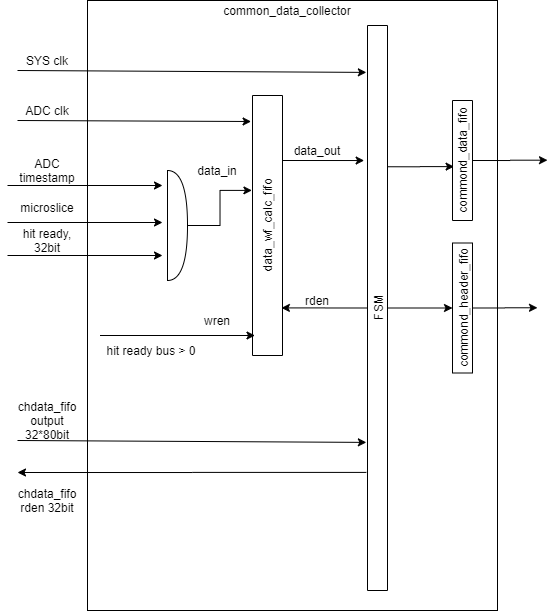
\includegraphics[width=0.5\textwidth]{ADC_common_event_collection.png}
	\caption{\label{fig:6} Data collecting scheme from all channels fifos}
\end{figure}


FSM is switched from wait to start state when data\_wf\_calc\_fifo\_isempty became '0' and fifo output is latched. Priority encoder show next fired channel from strobe and data collected from fired channel to common\_data\_fifo with hit\_packet\_iterator. Input to priory encoder is shifted to bit after fired channel when iterator reach last fired channel. Priority encoder could be equal or less than 32 bit. Simulation outputs presented on figure ~\ref{fig:4}.

\begin{figure}[H]
	\centering 
	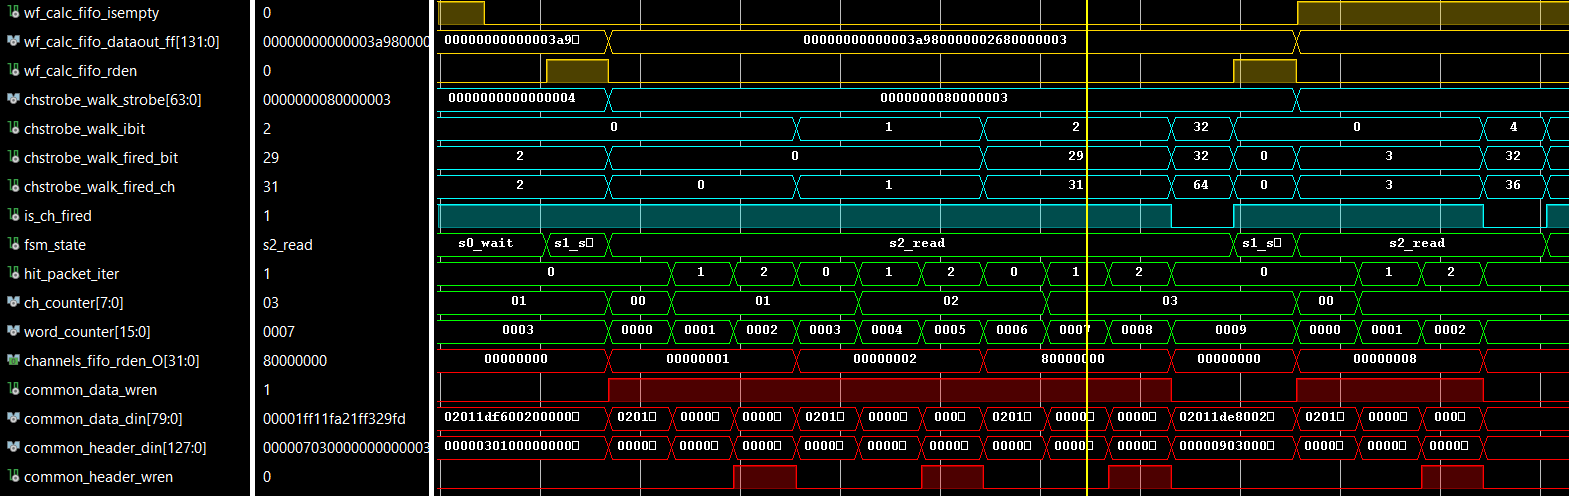
\includegraphics[width=1.0\textwidth]{ADC_common_data_collector_wave.png}
	\caption{\label{fig:7} Data collecting signal from all channels fifos}
\end{figure}

Collecting data from all channels takes two additional FSM cycle. Mean hit rate per channel in case all channels fired is SYSCKL / total channels + 2 cycle / packet length. Test beam: 80MHz / 12 / 5 = 1.3MHz. Final setup: 120 (240) / 32 / 1 = 3.5 (7) MHz.


\subsection{Component GBT\_data\_sender}

Data stored in common\_data\_fifo in component common\_data\_collector are read by system clock with writing rate. Event and microslice headers are formed by data from common\_header\_fifo. Built GBT data packets are stored in gbt\_data\_fifo and read by GBT TX clock. Signal diagram is presented on figure~\ref{fig:8}. 


\begin{figure}[H]
	\centering 
	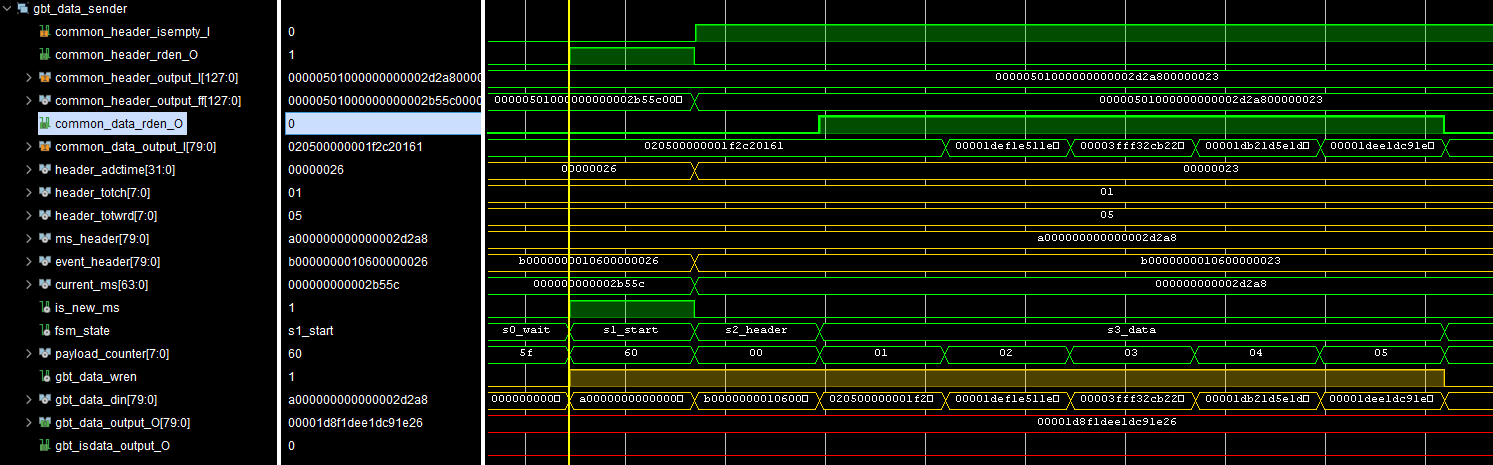
\includegraphics[width=1.0\textwidth]{GBT_sender_wave.png}
	\caption{\label{fig:8} Channel data collecting signals}
\end{figure}



Data rate limit is 80bit X 40MHz = 0.4 GB/s(GBT). Hit rate limit per channel (without microslice word) is 40MHz / 33 (packet length) = 1,2 MHz in case all channels are fired. The rate could be increased to  2.4 MHz hits per channel in case all 32 channels are fired. If one hit data will be less than 40bit event packet will contain 17 GBT words.

GBT packet format is presented on tables: ~\ref{tab1}, ~\ref{tab2}, ~\ref{tab3}





\begin{table}[H]
\centering
\begin{tabular}{| l | l | l | l | l | l | l | l | l |}
\hline
word type & 79 .. 76 & 75 .. 72 & 71 .. 64 & 63 .. 48 & 47 .. 40 & 39 .. 32 & 31 .. 16 & 15 .. 0 \\ \hline
ms header & 0xA & \multicolumn{2}{c|}{0x0}  & \multicolumn{5}{c|}{ms index} \\ \hline
event header & 0xB & ADC idx** & \multicolumn{2}{c|}{0x0} & n fired channels & words in packet * & \multicolumn{2}{c|}{adc time} \\ \hline
hit header & \multicolumn{8}{c|}{hit header (tab.~\ref{tab1})} \\ \hline
hit data & \multicolumn{8}{c|}{hit data (tab.~\ref{tab2})} \\ \hline
hit data & \multicolumn{8}{c|}{hit data (tab.~\ref{tab2})} \\ \hline
hit data & \multicolumn{8}{c|}{hit data (tab.~\ref{tab2})} \\ \hline
hit data & \multicolumn{8}{c|}{hit data (tab.~\ref{tab2})} \\ \hline
  & \multicolumn{8}{c|}{ ... } \\ \hline

event header & 0xB & ADC idx** & \multicolumn{2}{c|}{0x0} & n fired channels & words in packet * & \multicolumn{2}{c|}{adc time} \\ \hline
  & \multicolumn{7}{c|}{ ... } \\ \hline

\end{tabular}
\caption{GBT data format. [* number of GBT words in event packet: event header + all hit packets] [** ADC board index] \label{tab1}}
\end{table}

\begin{table}[H]
\centering
\begin{tabular}{| l | l | l | l | l | l |}
\hline
word & 79 .. 72 & 71 .. 64 & 63 .. 36 & 35 .. 16 & 15 .. 0 \\ \hline
1 & channel &words in packet *& 0x0 & signal charge & waveform zero level \\ \hline
\end{tabular}
\caption{hit packet header. [* total GBT words in hit packet: header + data words]\label{tab2}}
\end{table}

\begin{table}[H]
\centering
\begin{tabular}{| l | l | l | l | l | l |}
\hline
word & 79 .. 64 & 63 .. 48 & 47 .. 32 & 31 .. 16 & 15 .. 0 \\ \hline
1 & 0x0 & waveform point n & waveform point n+1 & waveform point n+2 & waveform point n+3 \\ \hline
\end{tabular}
\caption{hit packet data word.\label{tab3}}
\end{table}


\section{ADC control}
\subsection{control registers}

To avoid configuration corruption while GBT link fail, register 31 is reserved for lock key word. Control registers are available for writing if register 31 is 0xafafafaf. Register 31 is always open for writing.

\begin{table}[H]
\centering
\begin{tabular}{| l | l | l | l | l | l | l | l | l | l | l |}
\hline
addr & 31 .. 30 & 29 .. 28 & 27 .. 24 & 23 .. 20 & 19 .. 16 & 15 .. 14 & 13 .. 12 & 11 .. 8 & 7 .. 4 & 3 .. 0 \\ \hline
0 & 0x0 & \multicolumn{4}{c|}{threshold ch1} & 0x0 & \multicolumn{4}{c|}{threshold ch0} \\ \hline
1 & 0x0 & \multicolumn{4}{c|}{threshold ch3} & 0x0 & \multicolumn{4}{c|}{threshold ch2} \\ \hline
2 & 0x0 & \multicolumn{4}{c|}{threshold ch5} & 0x0 & \multicolumn{4}{c|}{threshold ch4} \\ \hline
3 & 0x0 & \multicolumn{4}{c|}{threshold ch7} & 0x0 & \multicolumn{4}{c|}{threshold ch6} \\ \hline
4 & 0x0 & \multicolumn{4}{c|}{threshold ch9} & 0x0 & \multicolumn{4}{c|}{threshold ch8} \\ \hline
5 & 0x0 & \multicolumn{4}{c|}{threshold ch11} & 0x0 & \multicolumn{4}{c|}{threshold ch10} \\ \hline
6 & 0x0 & \multicolumn{4}{c|}{threshold ch13} & 0x0 & \multicolumn{4}{c|}{threshold ch12} \\ \hline
7 & 0x0 & \multicolumn{4}{c|}{threshold ch15} & 0x0 & \multicolumn{4}{c|}{threshold ch14} \\ \hline
8 & 0x0 & \multicolumn{4}{c|}{threshold ch17} & 0x0 & \multicolumn{4}{c|}{threshold ch16} \\ \hline
9 & 0x0 & \multicolumn{4}{c|}{threshold ch19} & 0x0 & \multicolumn{4}{c|}{threshold ch18} \\ \hline
10 & 0x0 & \multicolumn{4}{c|}{threshold ch21} & 0x0 & \multicolumn{4}{c|}{threshold ch20} \\ \hline
11 & 0x0 & \multicolumn{4}{c|}{threshold ch23} & 0x0 & \multicolumn{4}{c|}{threshold ch22} \\ \hline
12 & 0x0 & \multicolumn{4}{c|}{threshold ch25} & 0x0 & \multicolumn{4}{c|}{threshold ch24} \\ \hline
13 & 0x0 & \multicolumn{4}{c|}{threshold ch27} & 0x0 & \multicolumn{4}{c|}{threshold ch26} \\ \hline
14 & 0x0 & \multicolumn{4}{c|}{threshold ch29} & 0x0 & \multicolumn{4}{c|}{threshold ch28} \\ \hline
15 & 0x0 & \multicolumn{4}{c|}{threshold ch31} & 0x0 & \multicolumn{4}{c|}{threshold ch30} \\ \hline
\end{tabular}
\caption{ADC channels threshold control.\label{tab4}}
\end{table}

\begin{table}[H]
\centering
\begin{tabular}{| l | l | l | l | l | l | l | l | l |}
\hline
addr & 31 .. 28 & 27 .. 24 & 23 .. 20 & 19 .. 16 & 15 .. 12 & 11 .. 8 & 7 .. 4 & 3 .. 0 \\ \hline
16 & \multicolumn{4}{c|}{0x0} & waveform length 0..3 [(reg+1)*4] & strobe offset 0..12 & \multicolumn{2}{c|}{control bits} \\ \hline
17 & \multicolumn{8}{c|}{negative channel mask ibit = ich} \\ \hline
\end{tabular}
\caption{ADC readout control.\label{tab5}}
\end{table}

\begin{table}[H]
\centering
\begin{tabular}{| l | l |}
\hline
bit & description \\ \hline
0 & send waveform \\ \hline
1 & ms gen standalone \\ \hline
2 & readout fsm reset \\ \hline
3 & errors reset \\ \hline
\end{tabular}
\caption{Control bits\label{tab6}}
\end{table}


\begin{table}[H]
\centering
\begin{tabular}{| l | l | l | l | l | l | l | l | l |}
\hline
addr & 31 .. 18 & 17 .. 17 & 16 .. 16 & 15 .. 8 & 7 .. 7 & 6 .. 0 \\ \hline
18 & 0x0 & WR & ENA & DATA & 0x0 & ADDR \\ \hline
\end{tabular}
\caption{HV control via I2C.\label{tab7}}
\end{table}


\section{CRI modules}
\subsection{ADC GBT emulator}

ADC GBT emulator generate GBT ADC packets filling hit packages with continuous hit counter. Parameters are:

\begin{itemize}
\item ms\_index - current microslice index @GBTclk to generate ms headers.


\item  event\_rate is number of GBT clock cycles between packets (from start to start). If previous packet was not sent, and is time to generate new one, new one skipped.

\item nch\_in\_even - number of hits per event 1 ... 32. Emulate fired channels.

\item hit\_packet\_len - number of hit packet words, including hit header 1 ... 5.

\end{itemize}

Emulator FSM is based on three counters, signals diagram is presented on figure \ref{fig:9}; generated data format is presented on figure \ref{tab8}.

\begin{figure}[H]
	\centering 
	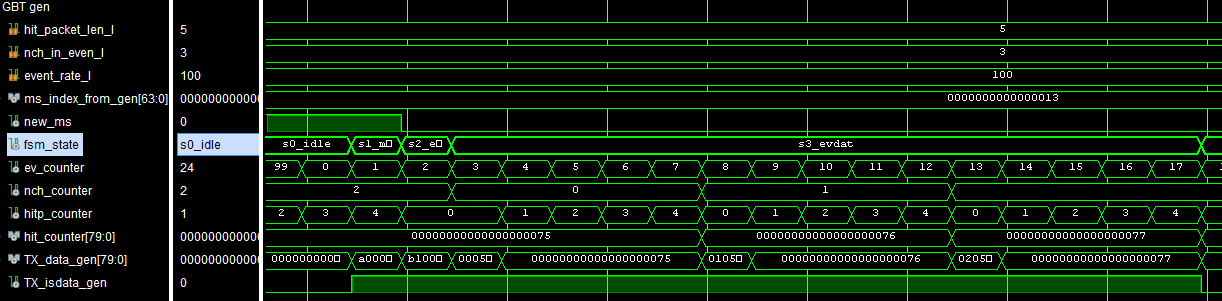
\includegraphics[width=1.0\textwidth]{ADC_GBT_emu_waves.png}
	\caption{\label{fig:9} ADC GBT emulator signals}
\end{figure}

\begin{table}[H]
\centering
\begin{tabular}{| l | l | l | l | l | l | l | l | l |}
\hline
word type & 79 .. 76 & 75 .. 72 & 71 .. 64 & 63 .. 48 & 47 .. 40 & 39 .. 32 & 31 .. 16 & 15 .. 0 \\ \hline
ms header & 0xA & \multicolumn{2}{c|}{0x0}  & \multicolumn{5}{c|}{ms index} \\ \hline
event header & 0xB & ADC idx** & \multicolumn{2}{c|}{0x0} & n hits & packet len * & \multicolumn{2}{c|}{0x0} \\ \hline
hit header & \multicolumn{2}{c|}{hit number} & words in hit packet *** & \multicolumn{5}{c|}{hit counter[63 .. 0]} \\ \hline
hit data & \multicolumn{8}{c|}{hit counter [79 ..0]} \\ \hline
hit data & \multicolumn{8}{c|}{hit counter [79 ..0]} \\ \hline
hit data & \multicolumn{8}{c|}{hit counter [79 ..0]} \\ \hline
hit data & \multicolumn{8}{c|}{hit counter [79 ..0]} \\ \hline
  & \multicolumn{8}{c|}{ ... } \\ \hline

event header & 0xB & ADC idx** & \multicolumn{2}{c|}{0x0} & n hits & packet len * & \multicolumn{2}{c|}{0x0} \\ \hline
  & \multicolumn{7}{c|}{ ... } \\ \hline

\end{tabular}
\caption{GBT data format. [* number of GBT words in event packet: event header + all hit packets] [** ADC board index] [*** total words in hit packet, including hit header]\label{tab8}}
\end{table}

\end{document}

